\section{Практическая часть}

{\color{red} Abstract}

\subsection{Цель}

С момента своей публикации, модель Трансформера \cite{vaswani2017attention}
завоевала огромное призвание. Однако у нее есть несколько серьезных 
проблем, которые усложняют работу с длинными временным последовательностями 
(LSTF). Последующие ислледования предложили различные методы решения 
данных и связующих проблем (см. Informer \cite{informer}, Performer \cite{performer}, 
Autoformer \cite{autoformer}, PatchTST \cite{patchTST}, TFT \cite{TFT} и др.). 
В данной работе мы сфокусируемся на первых трех.

В данной работе, мы предлагаем заменить слой эмбеддинга в модели 
Informer компактным двухслойным сверточным блоком с целью повышения 
эффективности извлечения локальных паттернов, внедрить модуль 
декомпозиции ряда из Autoformer для явного разделения 
трендовых и сезонных компонент и заменить ProbSparse-внимание 
на линейное FAVOR+ из Performer для учёта глобальных 
зависимостей при низких вычислительных затратах.

\subsection{Используемые данные}

Прежде чем перейти к методологии нашей работы, рассмотрим 
модели и понятия, которыми далее будем пользоваться.

\subsubsection{Informer}

В 2020 году, Zhou et al., опубликовали свою статью 
«\textbf{Informer: Beyond Efficient Transformer for 
Long Sequence Time-Series Forecasting}», в которой 
представили новую, основанную на Трансформере \cite{vaswani2017attention} 
модель под названием \textbf{Informer} \cite{informer}. 

\begin{figure}[h!]
    \centering
    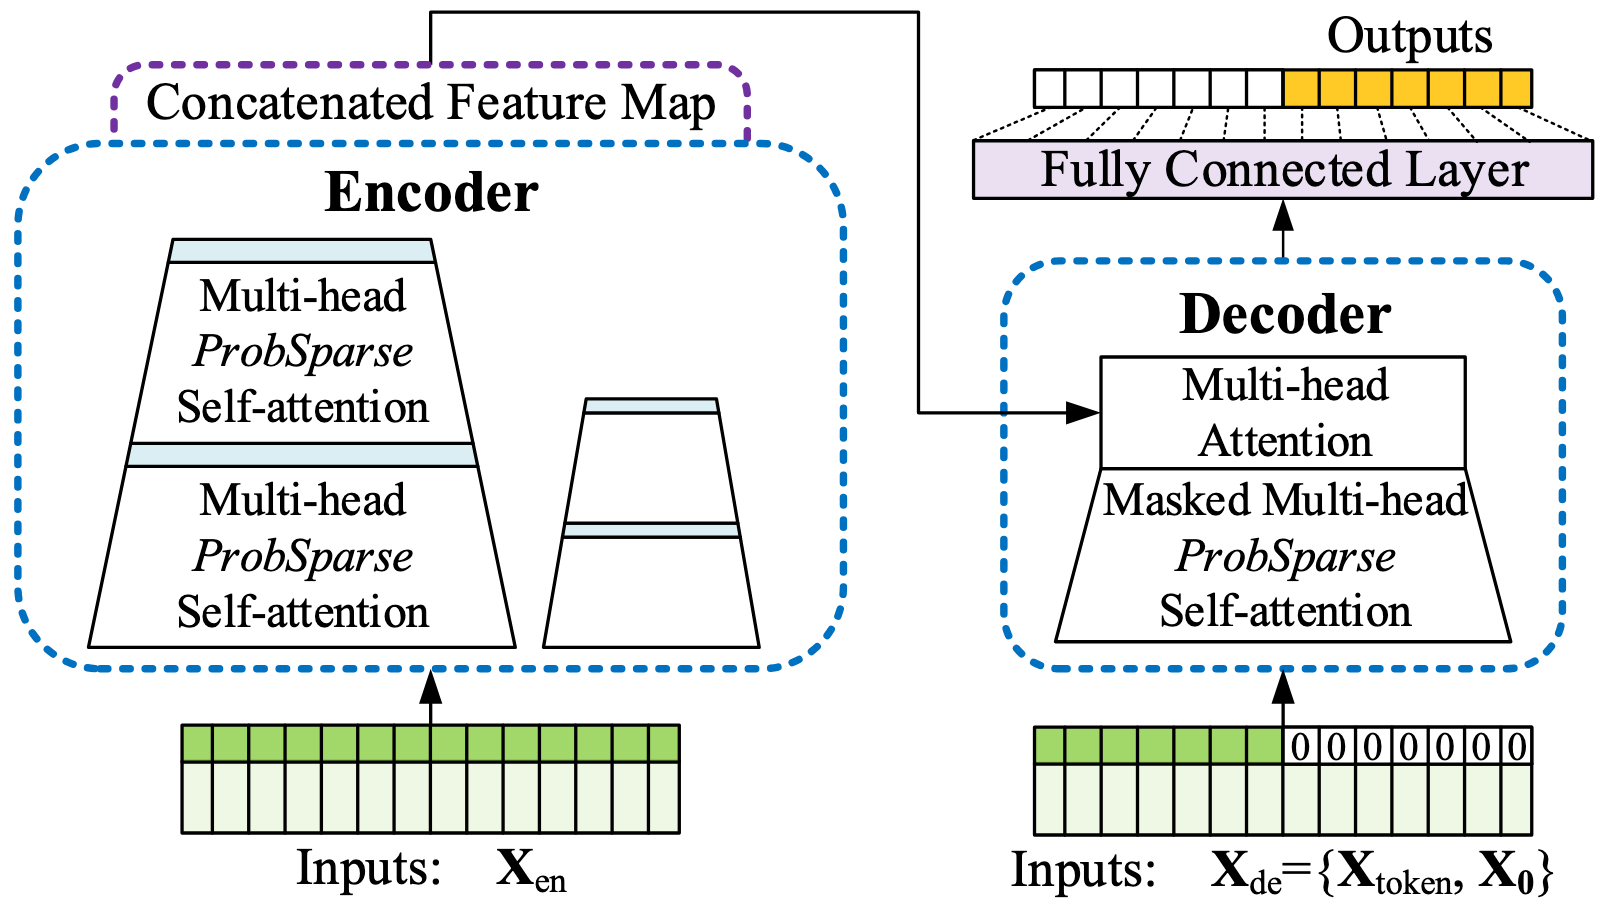
\includegraphics[width=0.8\textwidth, keepaspectratio]{informer}
    \caption{Обзор модели Informer \cite{informer}.}
    \label{fig:informer}
\end{figure}

Informer был создан для решения задачи 
\textbf{Long-sequence time-series forecasting (LSTF)}. 
Zhou et al. поставили перед собой следюущий вопрос: 
Можем ли мы построить модель, основанную на трансформере, 
которая 
\begin{enumerate}[label=(\alph*)]
    \item захватывает очень длинные зависимости
    \item эффективно работает для тысячи временных шагов
\end{enumerate}
Ключевые рассматриваемые слабости трансформера:
\begin{itemize}
    \item Квадратичная стоимость механизма само-внимания (self-attention) 
    для последовательностей длины $L$.
    \item Накладывание слоев умножает эту стоимость, достигая ограничений по памяти.
    \item Пошаговое (динамичное) декодирование работает медленно и накапливает ошибки. 
\end{itemize}

Информер отвечает на каждый из этих вопросов, реконструируя 
механизм внимания, кодировщик и декодер.

\paragraph{ProbSparse Self-Attention}

Зачастую, в длинных временных рядах, большинство 
скалярных произведений запросов с ключами пренебрежимо малы 
и лишь некоторые из них достаточно больши. 
Вместо того, чтобы считать все возможные пары запрос-ключ, 
informer предлагает следующее:
\begin{enumerate}
    \item Измерить разброс каждого запроса $q_i$:
    \begin{equation*}
        M(\bm{q}_i, \bm{K}) = \text{max}_j \cfrac{\bm{q}_i \bm{k}_j^T}{\sqrt{d}} - 
        \cfrac{1}{L_K} \sum_{j=1}^{L_K} \cfrac{\bm{q}_i \bm{k}_j^T}{\sqrt{d}}, 
    \end{equation*}
    \item Выбрать $u$ лучших запросов, исходя из $M(\bm{q}_i, \bm{K})$, 
    где $u \propto \ln L$.
    \item Вычислить полное внимание только для этих $u$ рядов и 
    аппроксимировать остальные через среднее значение.
\end{enumerate}
Что сокращает как время, так и память c $O(L^2)$ до $O(L \text{log} L)$, 
при этом сохраняя всю важную информацию.

\paragraph{Self-Attention Distilling \& Кодировщик}

Даже после предыдщей операции, каждый слой все равно производит 
карты признаков длины $L$, многие из которых повторяют похожие паттерны. 
Мы можем «дистиллировать» сильнейшие сигналы и сократить последовательность 
по мере продвижения.

\begin{itemize}
    \item После каждого блока с механизмом внимания, применяем:
    \begin{enumerate}
        \item 1-D свертку + ELU активацию, 
        \item max-pool со страйдом 2 
    \end{enumerate}
\end{itemize}
Что уменьшает размерность в два раза на каждом слое, результируя 
в пирамиде стэков, чьи выходы в конечном итоге конкатенируют. 

Self-attention distilling фокусируется на доминирующих паттернах, 
при этом сокращая память до $O((2-\varepsilon)L \log L)$.

\begin{figure}[h!]
    \centering
    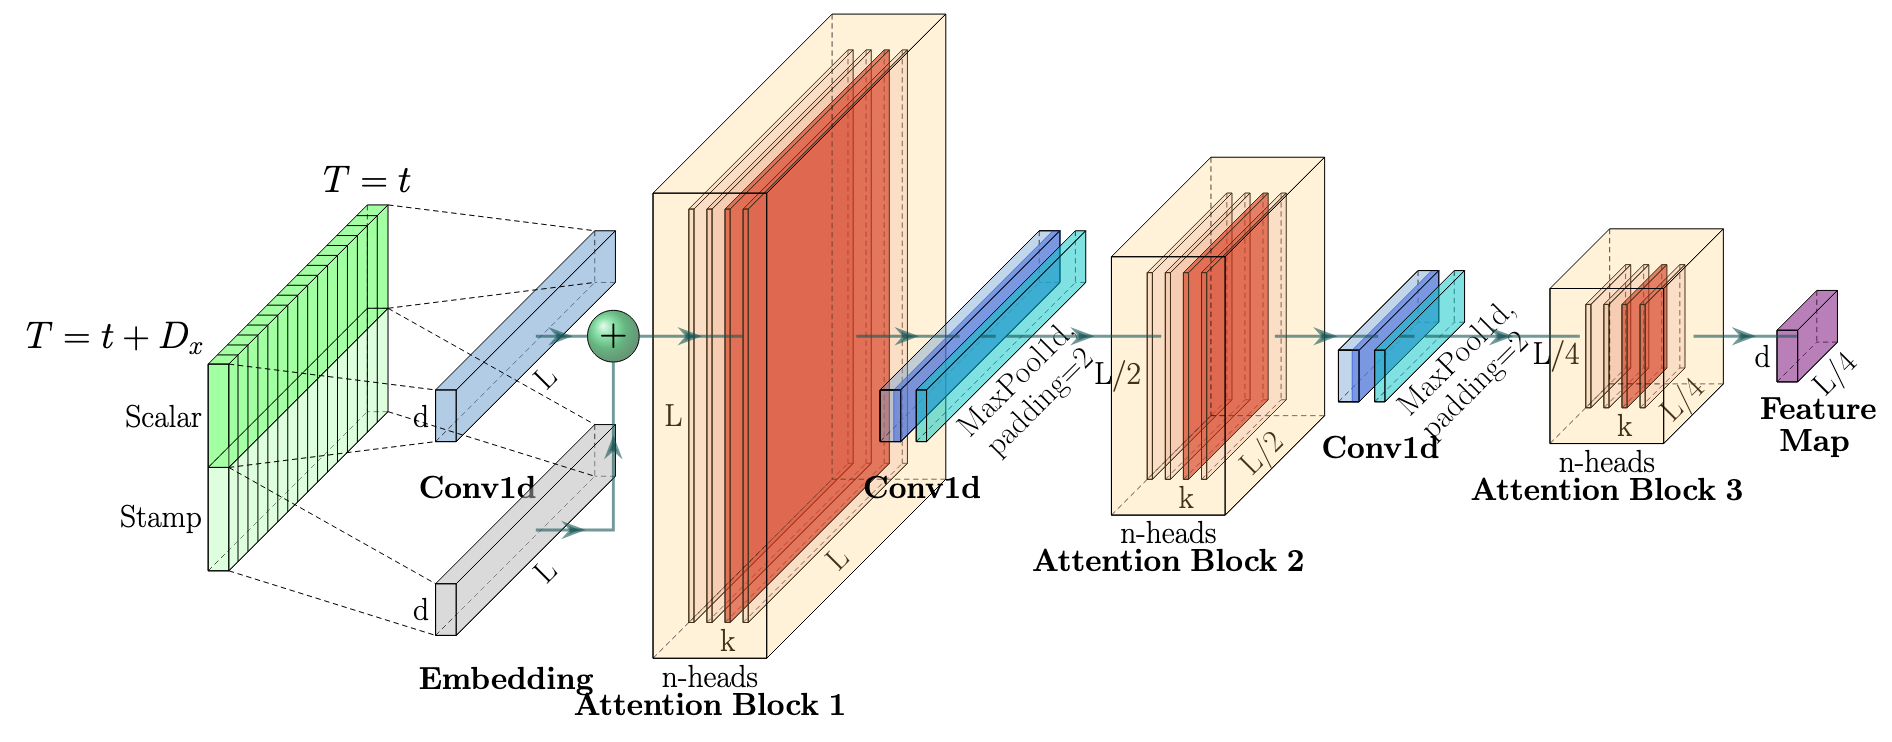
\includegraphics[width=1\textwidth, keepaspectratio]{informer_encoder}
    \caption{Обзор одного стэка в кодировщике Informer-а \cite{informer}.}
    \label{fig:informer_encoder}
\end{figure}

\paragraph{Генеративный декодер}

Вместо того, чтобы генерировать генерировать токены по очереди 
один за одним, заимствуем трюк с начальными токеном из NLP:
\begin{itemize}
    \item Взять срез ивестной истории (например 5 дней перед целевыми 7ю днями) в качесвте начального токена
    \item Разместить плейсхолдеры для всех $L_y$ будущих значение (используя только их временные метки для позиционного контекста)
    \item За один прямой проход одновременно заполнить все $L_y$ выходов через маскированное ProbSparse внимание.
\end{itemize} 
Что избегает накапливания ошибки и работает гораздо быстрее.

\subsubsection{Performer}

В 2020 году, Choromanski et al., опубликовали статью 
«\textbf{Rethinking Attention with Performers}», в которой 
переработали устройство механизма внимания в классических Трансформерах 
\cite{performer}. 

Как уже было сказано в главе выше, одной из ключевых проблем Трансформера 
являеется квадратичная сложность расчета внимания: $O(L^2)$. В своей работе, 
Choromanski et al. задались вопросом:
\begin{center}
    \itshape
    Можем ли мы добиться той же гибкости глобального внимания, но за линейное время и память?
\end{center}

\paragraph{FAVOR+: Fast Attention via positive Orthogonal Random features}

Вспомним, что в классическом Трансформере \cite{vaswani2017attention} 
внимание рассчитывается по следующей формуле (без учета нормирующей константы):
\begin{equation*}
    \text{Attention}(Q, K, V) = \text{softmax}(QK^T)V
\end{equation*}

Заметим, что
\begin{equation*}
    \text{exp}(q_i^T k_j) = \kappa (q_i, k_j),
\end{equation*}
где $\kappa$ - softmax ядро.

Согласно «\textbf{ядерному трюку}», мы можем представить $\kappa$ в виде:
\begin{equation*}
    \kappa(q_i, k_j) = \langle \phi(q_i), \phi(k_j) \rangle,
\end{equation*}
где $\phi$ - некоторое (возможно, высоко- или бесконечно-мерное) отображение признаков.

Что, в свою очередь, мы можем аппроксимировать согласно \textbf{random features}:
\begin{equation*}
    \kappa(q_i, k_j) \approx \langle \widetilde{\phi}(q_i), \widetilde{\phi}(k_j) \rangle
\end{equation*}

Performer предлагает \textbf{FAVOR+}, объединяющий в себе две идеи:
\begin{enumerate}
    \item \textbf{Positive Random Features (PRF)}: Вместо классических тригонометрических random features (которые могут принимать отрицательны значения), предлагается использовать отображение, основанное на экспоненте (таким образом все зачения будут неотрицательными).
    \item \textbf{Orthogonal Random Features (ORF)}: Выбирать случайные проекции так, чтобы они были взаимно ортогональными, а не независимыми (что уменьшает дисперсию).
\end{enumerate}

Откуда мы получаем выражение для $\phi$:
\begin{equation*}
    \phi(\bm{x}) = \cfrac{1}{\sqrt{m}} \ \text{exp} \left( \bm{W} \bm{x} - \frac{1}{2} || \bm{x} ||^2 \right),
\end{equation*}
где $\omega_i \sim \mathrm{N}(0, \bm{I}_d)$ - случайные ортогональные Гауссовы вектора 
(строки матрицы $\bm{W} = [\omega_1^T \ \omega_2^T ... \omega_m^T]^T$), 
$m$ - кол-во случайных признаков (размерность $\phi(\bm{x})$).

Обозначив $\Phi_Q = \phi(Q) \in \mathbb{R}^{L \times m}$ и $\Phi_K = \phi(K) \in \mathbb{R}^{m \times d}$, 
получаем:
\begin{equation*}
    \text{Attention}(Q,K,V) = \Phi_Q (\Phi_K^T V) \in \mathbb{R}^{L \times d},
\end{equation*}
где расчет $\Phi_Q$ и $\Phi_K$ занимает $O(L m d)$, 
расчет $\Phi_K^T V$ занимает $O(L m d)$, 
перемножение с $\Phi_Q$ занимает $O(L m d)$. 

Итого имеем линейную сложность для расчета внимания (памяти также требуются только 
эти три матрицы).

\subsubsection{Autoformer}

В 2021 году, Wu et al., опубликовали статью 
«\textbf{Autoformer: Decomposition Transformers with
Auto-Correlation for Long-Term Series Forecasting}», 
в которой представили новую модель, основанную на Трансформере - 
Autoformer с целью долгосрочного прогнозирования временных рядов. 
Auformer объединяет в себе автоматизированную 
декомпозицию временного ряда и новый механизм внимания, 
основанный на автокорреляции \cite{autoformer}.

В данной работе мы рассмотрим только часть с декомпозицией. 

\paragraph{Декомпозиция временого ряда}

В классическом анализе временных рядов (например 
декомпозиция по сезонным трендам с помощью LOESS), 
декомпозиция обычно рассматривается как процесс 
предобработки. Часто применяется скользящее среднее 
(здесь и далее под скользящим средним подразумеваем 
Simple Moving Average (SMA)) для извлечения тренда 
и сезонности из прошлого ряда, после чего остаток 
подается на вход модели. Однако после предобработки 
мы теряем возможность позволить модели 
уточнить или скорректировать эту декомпозицию 
по мере обработки более глубоких слоев.

Autoformer предлагает внедрить механизм декомпозиции 
в саму модель. Таким образом она сможет самостоятельно 
разделять тренд и сезонные компоненты ряда в каждом слое.

\begin{figure}[h!]
    \centering
    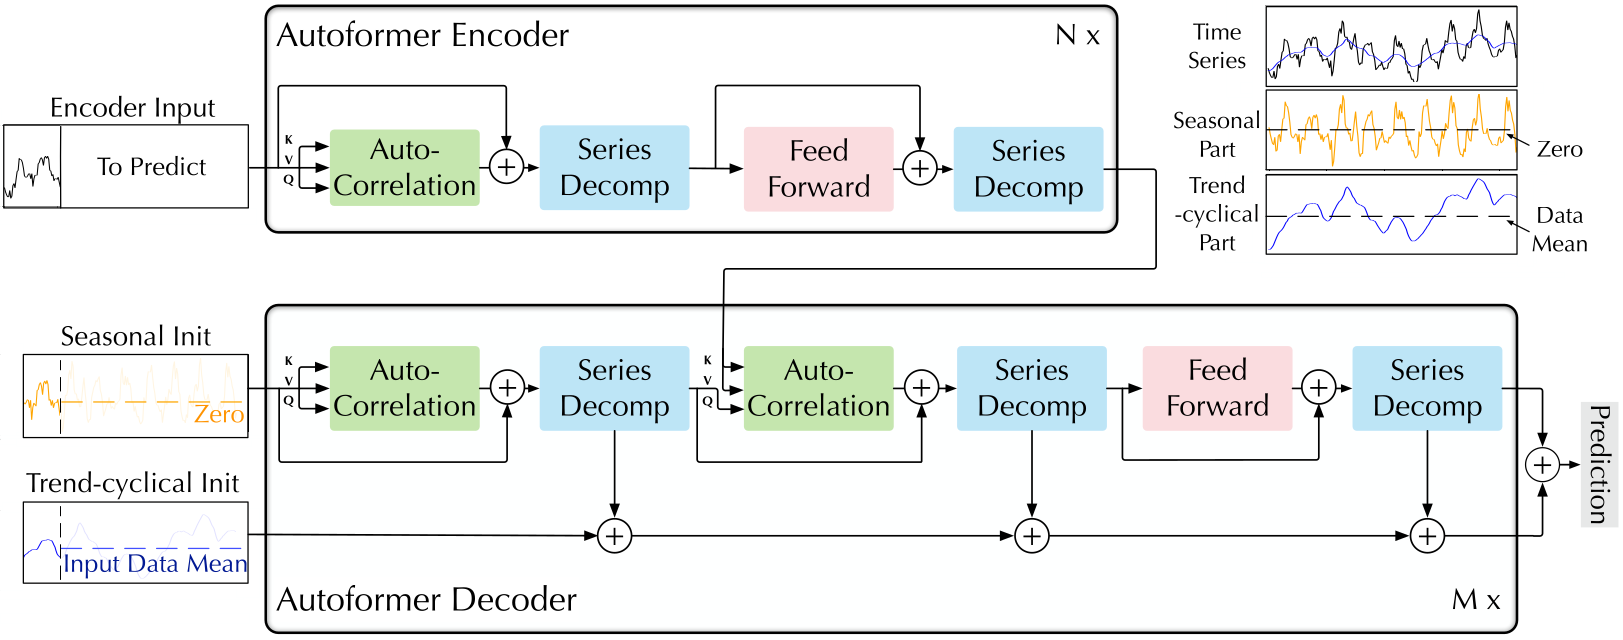
\includegraphics[width=1\textwidth, keepaspectratio]{autoformer}
    \caption{Архитектура Autoformer-а \cite{autoformer}.}
    \label{fig:autoformer}
\end{figure}

\newpage

На каждом слое $l$ берется входная последовательность 
(которая уже могла быть частитично обработана предыдущими слоями), 
к которой, внутри слоя, применяется скользящее среднее, что далее 
разделяется на две части:
\begin{itemize}
    \item $\text{Trend}^{(l)} = \text{SMA}(\text{Input}^{(l)})$
    \item $\text{Seasonal}^{(l)} = \text{Input}^{(l)} - \text{Trend}^{(l)}$
\end{itemize}

После чего мы передаем $\text{Seasonal}^{(l)}$ в наш механизм 
внимания, а $\text{Trend}^{(l)}$ направляем на вход в следующий слой 
(via residual connection). Схематично это можно изобразить 
следующим образом:

\begin{framed}
    \noindent Input: $\text{H}^{(l-1)}$ \\
    
    \noindent (1) [SeriesDecomp] $\rightarrow$ $\text{Trend}^{(l)}$, $\text{Seasonal}^{(l)}$ 
    
    \qquad where \vspace{-40pt} \begin{align*}
        & \text{Trend}^{(l)} = \text{SMA}(\text{H}^{(l-1)}) \\ 
        & \text{Seasonal}^{(l)} = \text{H}^{(l-1)} - \text{Trend}^{(l)} 
    \end{align*}

    \noindent (2) [selft-attention mechanism] on $\text{Seasonal}^{(l)}$

    \qquad $\rightarrow$ $\text{Seasonal}'^{(l)}$ (+ residual connection, normalization, etc.) \\ 

    \noindent (3) [Feed-Forward] on $\text{Seasonal}'^{(l)} \rightarrow \widetilde{\text{Seasonal}}^{(l)}$ \\
    
    \noindent (4) Re-compose $\text{H}^{(l)} = \widetilde{\text{Seasonal}}^{(l)} + \text{Trend}^{(l)}$
\end{framed}

\subsection{Методология}

% Informer + Conv-stem + SeriesDecomp (from Autoformer) + FAVOR+ (from Performer)
{\color{red} Informer + Conv-stem + SeriesDecomp (from Autoformer) + FAVOR+ (from Performer)}

\subsubsection{Повышение эффективности извлечения локальных паттернов}

В своей модели, мы предлагаем заменить TokenEmbedding внутри Embdding слоя 
в модели Informer двумя сверточными слоями, при этом оставив PositionalEmbedding 
и TemporalEmbedding (рис. \ref{fig:convstem}).

\begin{figure}[h!]
    \centering
    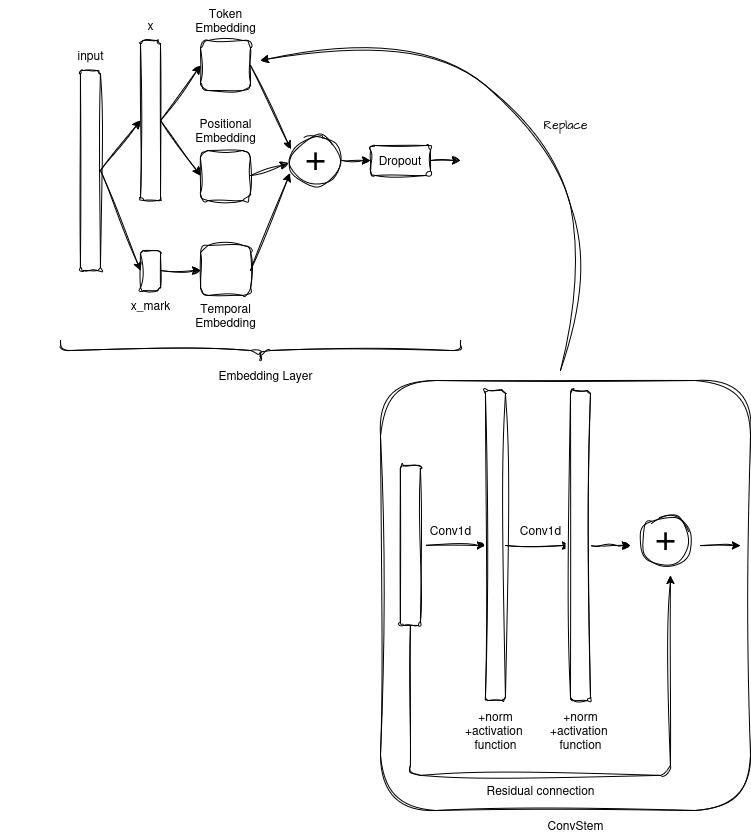
\includegraphics[width=0.7\textwidth, keepaspectratio]{ConvStem.png}
    \caption{Схема замены TokenEmbedding внутри Embdding слоя в Informer на ConvStem. 
    ConvStem состоит из двух последовательных операций свертки, первая из которых 
    отображает признаки в размерность модели, вторая не изменяет размерность. В 
    качестве нормализации была выбрана Instance normalization, в качестве функции активации 
    - GELU. Также было добавлено residual connection. Реализацию см. в \ref{lst:convstem}.}
    \label{fig:convstem}
\end{figure}

Данную замену мы мотивируем тем, что компактный двухслойный сверточный блок 
обеспечивает явную индуктивную привязку к локальным временным паттернам и 
относительным позициям без необходимости в дополнительных позиционных кодировках, 
позволяя механизмам глобального внимания сконцентрироваться на долгосрочных зависимостях. 
Кроме того, ConvStem существенно снижает число параметров и вычислительную нагрузку 
по сравнению с классическим TokenEmbedding, что критично при ограниченных ресурсах GPU.

\subsubsection{Заимствование механизма внимания из Performer}

В качестве механизма внимания предлагается использовать FAVOR+ 
(из Performer) вместо ProbSparse (оригинально используемого в Informer).

Подобно тому, как в оригинальном Informer механизм FullAttention был заменен на 
ProbSparse исключительно для вычисления self-attention в слоях кодировщика и 
декодера, в нашей модификации ProbSparse будет заменен на FAVOR+ в тех же местах, 
тогда как cross-attention останется реализованным через FullAttention. 
Реализацию см. в \ref{lst:favor}.

% probsparse self-attention from informer -> FAVOR+ from performer
% leave corss-attention as is?

\subsubsection{Внедрение модуля декомпозиции ряда из Autoformer}

% -----

% put here full end architecture

\subsection{Эксперимент}

\subsubsection{Датасет}

В данной работе мы проводим эксперименты на датасете 
(\textbf{Electricity Transformer Temperature}) \cite{informer}:
ETT является важнейшим индикатором долгосрочного развертывания 
электроэнергетики. Создатели Informer собрали данные за 
2 года из двух отдельных уездов Китая. Датасет разбит на несколько 
частей: \{ ETTm1, ETTm2 \}, где данные записаны по-минутно, а 
также \{ ETTh1, ETTh2 \}, где данные записаны по-часово 
для быстрой разработки. Каждый элемент данных состоит из 
8 признаков, включая дату измерения, целевую переменную 
"температура масла" и 6 различных видов признаков внешней силовой 
нагрузки.  

\begin{figure}[h!]
    \centering
    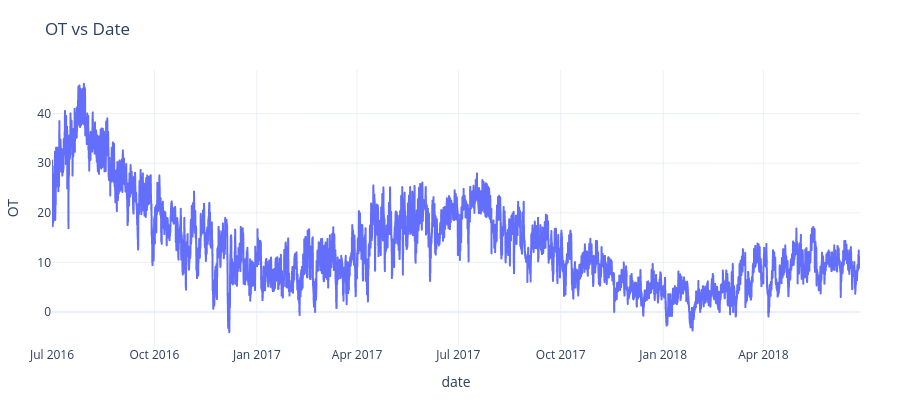
\includegraphics[width=1\textwidth, keepaspectratio]{ETT_OTvsDATE}
    \caption{Общий вид «ОТ» в ETT-small \cite{informer}.}
    \label{fig:ETT_OTvsDATE}
\end{figure}

\begin{figure}[h!]
    \centering
    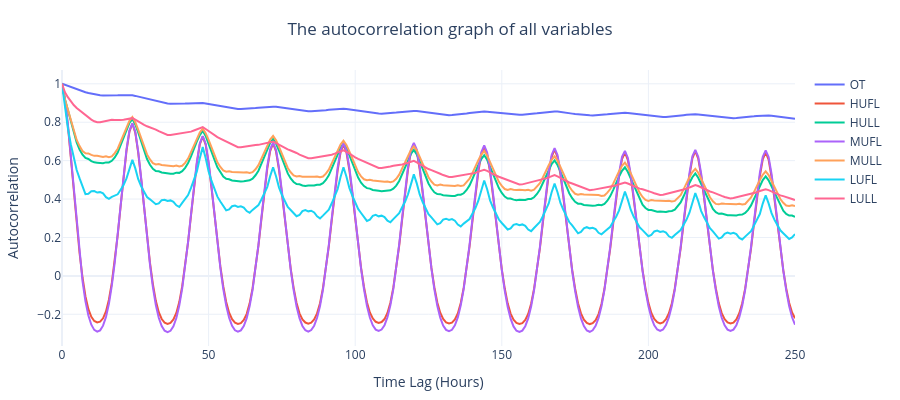
\includegraphics[width=1\textwidth, keepaspectratio]{ETT_autocorrelation}
    \caption{График автокорреляции всех переменных \cite{informer}.}
    \label{fig:ETT_autocorrelation}
\end{figure}

\begin{table}[h!]
    \centering
    \begin{adjustbox}{max width=1\textwidth}
    \setlength{\tabcolsep}{20pt} % Increase horizontal space between columns
    \begin{tabular}{ 
          c       % first column centered
          !{\vrule width 1pt}  % thick vertical line
          c c c c c c c c       % eight more centered columns
        }
        \toprule
        % Header row: each entry is centered and single‐line,
        % so we can just write them normally.
        \makecell{\textbf{Field}} 
          & \makecell{\textbf{date}} 
          & \makecell{\textbf{HUFL}} 
          & \makecell{\textbf{HULL}} 
          & \makecell{\textbf{MUFL}} 
          & \makecell{\textbf{MULL}} 
          & \makecell{\textbf{LUFL}} 
          & \makecell{\textbf{LULL}} 
          & \makecell{\textbf{OT}} 
        \\
        \midrule
        % Second row: force each word onto its own line using \makecell{…}
        \makecell{Description} 
          & \makecell{The\\recorded\\\textbf{date}} 
          & \makecell{\textbf{H}igh\\\textbf{U}se\textbf{F}ul\\\textbf{L}oad} 
          & \makecell{\textbf{H}igh\\\textbf{U}se\textbf{L}ess\\\textbf{L}oad} 
          & \makecell{\textbf{M}iddle\\\textbf{U}se\textbf{F}ul\\\textbf{L}oad} 
          & \makecell{\textbf{M}iddle\\\textbf{U}se\textbf{L}ess\\\textbf{L}oad} 
          & \makecell{\textbf{L}ow\\\textbf{U}se\textbf{F}ul\\\textbf{L}oad} 
          & \makecell{\textbf{L}ow\\\textbf{U}se\textbf{L}ess\\\textbf{L}oad} 
          & \makecell{\textbf{O}il\\\textbf{T}emperature\\(target)} 
        \\
        \bottomrule
    \end{tabular}
    \end{adjustbox}
    \caption{Описание каждого столбца.}
    \label{tab:columns_description}
\end{table}

% Brief summary of ETT-h1 (70 k rows, 8 vars, horizons)
% Forecasting setup (seq = 168, pred ∈ {96,192,336,720})

\subsubsection{Benchmark}

% DONT FORGET MAPE 
% results for the full hybrid model

\subsubsection{Детали}

\textbf{Baselines:} {\color{red} todo}
\textbf{Setup:} Входные данные каждого набора данных нормализованы по нулевому среднему значению. 
Согласно устройству LSTF, мы постепенно увеличиваем размер горизонта предсказаний, 
т.е. \{ 1d, 2d, 7d, 14d, 30d, 40d \}.
\textbf{Metrics:} Мы пользуемся двумя метриками оценки, включая 
$\text{MSE}=\frac{1}{n} \sum_{i=1}^n (\bm{y} - \hat{\bm{y}})^2$ 
и $\text{MAE}=\frac{1}{n} \sum_{i=1}^n |\bm{y} - \hat{\bm{y}}|$ 
для каждого из горизонтов предсказаний (усредняя для многомерного 
предсказания), и прогоняем весь набор с stride=1.
\textbf{Platform:}
Все модели были тренированы/тестированы на единственной 
NVIDIA GTX 1660 SUPER GPU. Исходный код доступен 
по ссылке: {\color{red} todo}.

\subsection{Ablations}

\subsubsection{Pure ConvStem}

Сравнение эффективности оригинальной модели Informer и модифицированной
с заменой TokenEmbedding внутри Embdding layer на ConvStem 
на метриках MSE \& MAE (таблица \ref{tab:etth1-convstem}).

\begin{table}[!ht]
    \centering
    \begin{tabular}{c  cc  cc}
    \toprule
    \multirow{2}{*}{{Horizon}} 
      & \multicolumn{2}{c}{{Informer}} 
      & \multicolumn{2}{c}{\textbf{ConvStem}} \\
    \cmidrule(lr){2-3} \cmidrule(lr){4-5}
      & {MSE} & {MAE} 
      & {MSE} & {MAE} \\
    \midrule
    24   & 0.556 & 0.547 & \textbf{0.503} & \textbf{0.504} \\
    48   & 0.657 & 0.614 & \textbf{0.578} & \textbf{0.548} \\
    168  & 0.862 & 0.725 & \textbf{0.853} & \textbf{0.720} \\
    336  & 1.219 & 0.892 & \textbf{1.132} & \textbf{0.861} \\
    720  & \textbf{1.183} & \textbf{0.871} & 1.247 & 0.912 \\
    \bottomrule
    \end{tabular}
    \caption{Результаты многомерных предсказаний на датасете ETTh1 с 
    горизонтами предсказаний: \{ 24, 48, 168, 336, 720 \}. 
    Мы фиксируем входную длину последовательностей у моделей как 96.
    Результаты были найдены в ходе усреднения по 10 отдельным запускам 
    для каждого из горизонтов.}
    \label{tab:etth1-convstem}
\end{table}

Было установлено, что при коротком горизонте предсказаний 
ConvStem превосходит Informer; с увеличением длины горизонта 
их результаты постепенно сравниваются, а при длинном горизонте 
ConvStem начинает уступать, что ожидаемо для сверточных механизмов.

\subsubsection{ProbSparse -> FAVOR+}

Сравнение эффективности оригинальной модели Informer и модифицированной
с заменой ProbAttention на FAVOR+ 
на метриках MSE \& MAE (таблица \ref{tab:etth1-favor}).

\begin{table}[!ht]
    \centering
    \begin{tabular}{c  cc  cc}
    \toprule
    \multirow{2}{*}{{Horizon}} 
      & \multicolumn{2}{c}{{Informer}} 
      & \multicolumn{2}{c}{with FAVOR+} \\
    \cmidrule(lr){2-3} \cmidrule(lr){4-5}
      & {MSE} & {MAE} 
      & {MSE} & {MAE} \\
    \midrule
    24   & 0.556 & 0.547 & 0.525 & 0.528 \\
    48   & 0.657 & 0.614 & 0.680 & 0.626 \\
    168  & 0.862 & 0.725 & 0.889 & 0.751 \\
    336  & 1.219 & 0.892 & 1.067 & 0.842 \\
    720  & 1.183 & 0.871 & 1.090 & 0.842 \\
    \bottomrule
    \end{tabular}
    \caption{Результаты многомерных предсказаний на датасете ETTh1 с 
    горизонтами предсказаний: \{ 24, 48, 168, 336, 720 \}. 
    Мы фиксируем входную длину последовательностей у моделей как 96.
    Результаты были найдены в ходе усреднения по 10 отдельным запускам 
    для каждого из горизонтов.}
    \label{tab:etth1-favor}
\end{table}

Было установлено, что на всех горизонтах предсказаний различия в результатах 
статистически незначимы, что ожидаемо, поскольку и ProbSparse ($O(L \log L)$ в среднем) 
и FAVOR+ (около $O(Lr)$ при $r \ll L$) направлены на ускорение классического механизма 
внимания ($O(L^2)$) при контролируемом уровне потерь в точности.

% we get to compare (a) vanilla Informer, (b) Informer + Performer, 
% (c) Informer + Performer + Autoformer‐decomp, and (d) a 
% “pure Autoformer” baseline—all within the same code framework.

% etc.

\subsection{Результаты}

% convstem показал себя лучше Informer при коротких горизонтах 
% предсказаний и хуже при длинных (что ожидаемо? тк мы работаем со свертками)

\subsection{Заключение}
